% Chapter Template

\chapter{Теоријска поставка} % Main chapter title

\label{Теоријска поставка} % Change X to a consecutive number; for referencing this chapter elsewhere, use \ref{ChapterX}

\lhead{Поглавље \thechapter. \emph{Теоријска поставка}} % Change X to a consecutive number; this is for the header on each page - perhaps a shortened title

...

\section{Хигс бозон у СМ}

\subsection{Хигс потенцијал и нарушење глобалне симетрије}

Хигс поље, илустровано на Сл.~\ref{fig:mexican_hat}, представља скаларни потенцијал у облику ''мексичког шешира''. Описано је једначином~(\ref{eq:V_higgs}) у којој се појављују чланови са имагинарном масом ($\mu^2 < 0$) и $\lambda > 0$.

\begin{equation}
V(\phi) = \mu^2(\phi^*\phi) + \lambda(\phi^*\phi)^2
\label{eq:V_higgs}
\end{equation}

\begin{figure}[H]
  \centering
	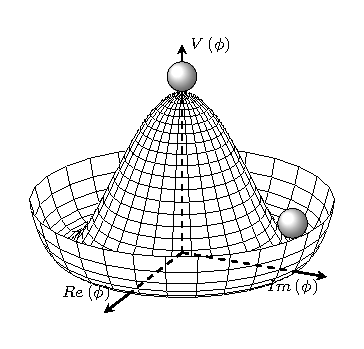
\includegraphics[width=0.505\textwidth]{texImages/mexican_hat.pdf}
	\caption{Облик Хигс потенцијала $V(\phi) = \mu^2(\phi^*\phi) + \lambda(\phi^*\phi)^2$, код којег су $\mu^2 < 0$ и $\lambda > 0$.}
	\label{fig:mexican_hat}
\end{figure}

...
